\section{Introduction}

As technology becomes an embedded part of everyday life and new trends such as the internet of things connect everyday objects to the internet, the amount of data stored in the digital universe has been growing at an outstanding rate. Consequently, processing and analyzing these datasets has become increasingly difficult and consequently multiple techniques have been developed in the fields of machine learning, data mining and others, to facilitate the use of this information.
% * <philip@thruesen.dk> 2016-05-31T20:43:13.004Z:
%
% > big data
%
% Is "big data" a field? Isn't it more "data mining" we should mention
%
% ^ <roelcastanomoreno@gmail.com> 2016-06-01T08:07:31.204Z:
%
% agree too
%
% ^ <jarekcechak@gmail.com> 2016-06-02T07:32:57.431Z.
% * <philip@thruesen.dk> 2016-05-31T20:36:18.745Z:
%
% perhaps "part of ALL human nature" is a pretty harsh opinion? What about "an embedded part of everyday life"
%
% ^ <roelcastanomoreno@gmail.com> 2016-06-01T08:07:14.174Z:
%
% agreed
%
% ^ <jarekcechak@gmail.com> 2016-06-02T07:33:07.172Z.

One of the many problems that arises from this growth in digital capacity is retrieving information in a form that is useful to the users. Simply retrieving relevant information is not enough, since it can span a significant amount of data. We can see examples of this with search engines, recommender systems, and bioinformatics, where it is necessary to provide users with the relevant data based on relevance to a certain query and sort it accordingly. The Learning to Rank algorithm is designed to solve this issue by taking into account multiple features which influence the relevance of each element and extensive research has been done to improve it over the past decade.

One interesting case where Learning to Rank (L2R) could be applied to is in determining the value of certain links in Wikipedia articles to help users better navigate the encyclopedia by preventing overlinking of articles. Wikipedia is an internet encyclopedia with more than 38 million articles in over 250 different languages of semi-structured information \cite{wikistats}. It is also the most popular wiki-based website, and is ranked by Alexa as the \#6 most popular website on the internet \cite{alexa}. It allows collaborative modifications of its articles by the users, which is one of the main reasons Wikipedia has grown to such an enormous size.
% * <philip@thruesen.dk> 2016-05-31T20:56:52.080Z:
%
% > which is one of the main reasons Wikipedia has grown to such an enormous size
%
% Probably also need source/reference on this
%
% ^ <roelcastanomoreno@gmail.com> 2016-06-02T07:46:40.923Z.
% * <philip@thruesen.dk> 2016-05-31T20:53:50.897Z:
%
% > Wikipedia is an internet encyclopedia with more than 38 million articles in over 250 different languages of semi-structured information. It is also the most popular wiki-based website
%
% Needs reference
%
% ^ <roelcastanomoreno@gmail.com> 2016-06-02T07:46:56.385Z.

\begin{figure}[H]
\centering
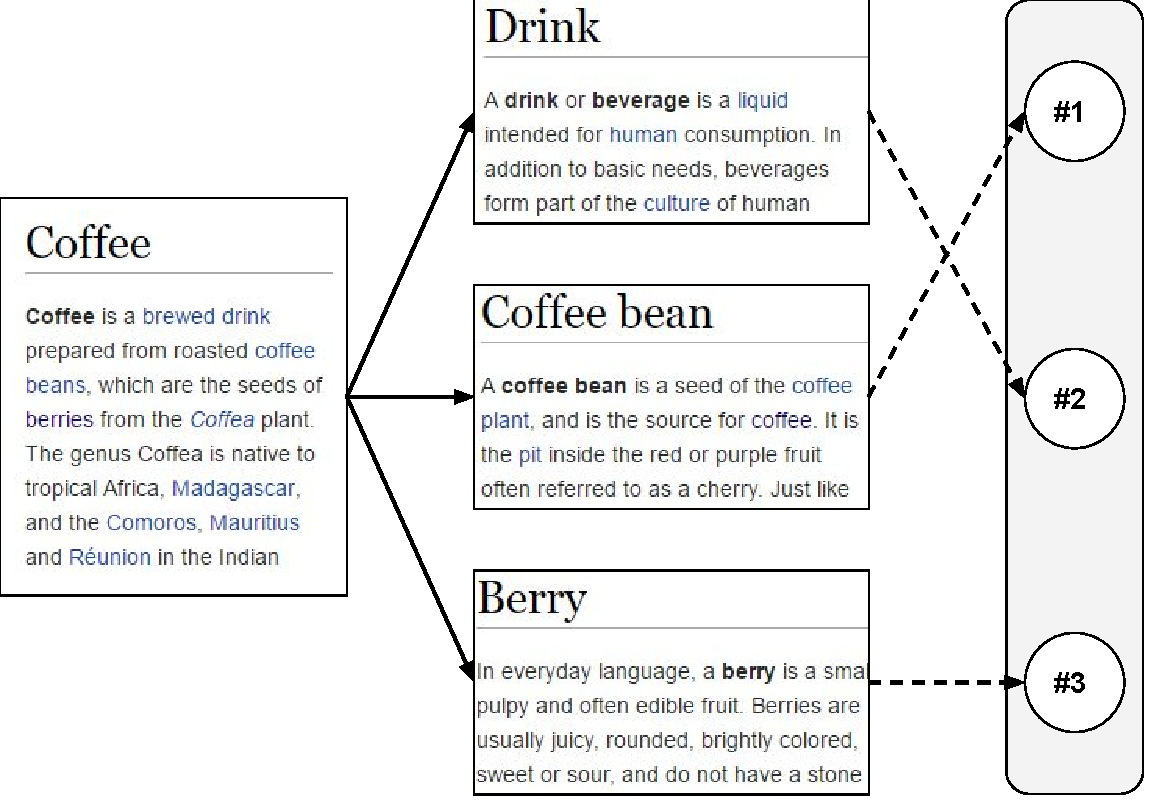
\includegraphics[width=0.49\textwidth]{images/concept}
	\caption{The main article, ``Coffee'', links to multiple articles including the 3 illustrated. These referenced articles, or more specifically, their links appearing in the main article, we attempt to rank according to predicted click frequency.} 
 \label{fig:concept}
\end{figure}
% * <philip@thruesen.dk> 2016-05-31T21:39:19.614Z:
%
% From here and to the end of the introduction I have a bunch of changes. - hope they make sense
%
% ^.
Being ``the free encyclopedia that anyone can edit'', as Wikipedia's slogan suggests, has many advantages and disadvantages where an example of the latter is \textit{overlinking}, further explained below. From an analysis by Ashwin Paranjape et al. \cite{paranjape}:  ``in the English Wikipedia, of all the 800,000 links added to the site in February 2015, the majority (66\%) were not clicked even a single time in March 2015, and among the rest, most links were clicked only very rarely''. Since most of the editing of articles is done manually, a lot of links are added based on individual author preferences which are not always strictly according to the Wikipedia Manual of Style \cite{lead} which recommend that you insert a link if it ``would help someone understand the article you are linking from''. 
% * <philip@thruesen.dk> 2016-05-31T22:42:11.254Z:
%
% The rest of the introduction is something I just added to reference the figure. Edit as you will.
%
% ^ <roelcastanomoreno@gmail.com> 2016-06-02T07:49:21.300Z.
By assuming a link is not helping anyone when not clicked over a significant amount of time we consider a problem of predicting the most valuable (and invaluable) links for the users. We approach this as a ranking problem having multiple features as input constructed on articles and their relations. Figure \ref{fig:concept} illustrates the concept of ranking referenced articles that appear as links in the article ``Coffee''. In this fictive example we predict ``Coffee bean' to be the most clicked and ``Berry'' the least. The bottom of this ranked list are potential candidates of links to be removed due to overlinking, however, our work only focuses on ranking and making such decisions is out of this article's scope. Having this in mind, we would like answer the following questions.
\begin{itemize}
\item Which features of the articles influence the click frequency of links the most?
% * <philip@thruesen.dk> 2016-05-31T21:43:39.678Z:
%
% > click frequency
%
% I changed value to 'click frequency'. I think its the most precise description. 'value' is pretty subjective.
%
% ^ <roelcastanomoreno@gmail.com> 2016-06-02T07:49:25.842Z.
\item To what extent can we use the L2R algorithm to predict relevance of links?
\item Can L2R help with reducing overlinking problem?
% * <jarekcechak@gmail.com> 2016-05-31T21:49:37.871Z:
%
% Is the third question OK? Can we answer it in the report?
%
% ^ <roelcastanomoreno@gmail.com> 2016-06-02T07:49:27.223Z.
\end{itemize}

